\documentclass[11pt]{article}
\usepackage{lmodern,float}
\usepackage{amssymb,amsmath}
\usepackage{ifxetex,ifluatex}
\usepackage{fixltx2e} % provides \textsubscript
\ifnum 0\ifxetex 1\fi\ifluatex 1\fi=0 % if pdftex
  \usepackage[T1]{fontenc}
  \usepackage[utf8]{inputenc}
\else % if luatex or xelatex
  \ifxetex
    \usepackage{mathspec}
  \else
    \usepackage{fontspec}
  \fi
  \defaultfontfeatures{Ligatures=TeX,Scale=MatchLowercase}
\fi
% use upquote if available, for straight quotes in verbatim environments
\IfFileExists{upquote.sty}{\usepackage{upquote}}{}
% use microtype if available
\IfFileExists{microtype.sty}{%
\usepackage{microtype}
\UseMicrotypeSet[protrusion]{basicmath} % disable protrusion for tt fonts
}{}
\usepackage[margin=1in]{geometry}
\usepackage{hyperref}
\hypersetup{unicode=true,
            pdftitle={Instructions/Worksheet},
            pdfauthor={NUS Statistics Enrichment Camp},
            pdfborder={0 0 0},
            breaklinks=true}
\urlstyle{same}  % don't use monospace font for urls
\usepackage{graphicx,grffile}
\makeatletter
\def\maxwidth{\ifdim\Gin@nat@width>\linewidth\linewidth\else\Gin@nat@width\fi}
\def\maxheight{\ifdim\Gin@nat@height>\textheight\textheight\else\Gin@nat@height\fi}
\makeatother
% Scale images if necessary, so that they will not overflow the page
% margins by default, and it is still possible to overwrite the defaults
% using explicit options in \includegraphics[width, height, ...]{}
\setkeys{Gin}{width=\maxwidth,height=\maxheight,keepaspectratio}
\IfFileExists{parskip.sty}{%
\usepackage{parskip}
}{% else
\setlength{\parindent}{0pt}
\setlength{\parskip}{6pt plus 2pt minus 1pt}
}
\setlength{\emergencystretch}{3em}  % prevent overfull lines
\providecommand{\tightlist}{%
  \setlength{\itemsep}{0pt}\setlength{\parskip}{0pt}}
\setcounter{secnumdepth}{5}
% Redefines (sub)paragraphs to behave more like sections
\ifx\paragraph\undefined\else
\let\oldparagraph\paragraph
\renewcommand{\paragraph}[1]{\oldparagraph{#1}\mbox{}}
\fi
\ifx\subparagraph\undefined\else
\let\oldsubparagraph\subparagraph
\renewcommand{\subparagraph}[1]{\oldsubparagraph{#1}\mbox{}}
\fi

%%% Use protect on footnotes to avoid problems with footnotes in titles
\let\rmarkdownfootnote\footnote%
\def\footnote{\protect\rmarkdownfootnote}

%%% Change title format to be more compact
\usepackage{titling}

% Create subtitle command for use in maketitle
\newcommand{\subtitle}[1]{
  \posttitle{
    \begin{center}\large#1\end{center}
    }
}

\setlength{\droptitle}{-2em}

  \title{Instructions/Worksheet}
    \pretitle{\vspace{\droptitle}\centering\huge}
  \posttitle{\par}
    \author{NUS Statistics Enrichment Camp}
    \preauthor{\centering\large\emph}
  \postauthor{\par}
      \predate{\centering\large\emph}
  \postdate{\par}
    \date{07 Jun 2019}


\begin{document}
\maketitle

\hypertarget{goals}{%
\section{Goals}\label{goals}}

In this exercise, we shall try to address the following questions by
collecting data on ourselves:

\begin{enumerate}
\def\labelenumi{\arabic{enumi}.}
\tightlist
\item
  Does resting heart rate differ according to gender, height and weight?
\item
  How much is heart rate affected by

  \begin{itemize}
  \tightlist
  \item
    watching an exciting sports video?
  \item
    working on a math problem?
  \end{itemize}
\item
  How long does it take our heart rate to recover after moderate amount
  of physical activity?
\end{enumerate}

As you proceed through this session, think about each step you are
doing. The following questions may be interesting to ask at each stage:

\begin{itemize}
\tightlist
\item
  Why are we using \emph{this} tool/program?
\item
  What do I expect to see happen?
\item
  What can I conclude from this output? Is the conclusion clear cut? Did
  I overlook any possibilities?
\end{itemize}

\hypertarget{setting-up}{%
\section{Setting Up}\label{setting-up}}

At any point, if you need help, please raise your hand.

\hypertarget{downloading-what-you-need}{%
\subsection{Programs That You Need}\label{downloading-what-you-need}}

\begin{enumerate}
\def\labelenumi{\arabic{enumi}.}
\tightlist
\item
  Log in to the PC in front of you. The user name (do not leave out the
  period and the backslash) and password are given on the whiteboard in front
of you.
\item
  All the files you need are inside a folder, on the Desktop, entitled
``stats\_camp'.
\item
  Open up the folder. It should contain the following items:
  \begin{enumerate}
  \def\labelenumii{\arabic{enumii}.}
  \tightlist
  \item
    hr2b.ino - a file that is been loaded onto the Arduino.
  \item
    data\_capture.ipynb - a Python notebook for data capture.
  \item
    math\_problem.pdf - a mathematics problem for you to solve.
  \end{enumerate}
\end{enumerate}

\hypertarget{arduino}{%
\subsection{Arduino}\label{arduino}}

\begin{enumerate}
\def\labelenumi{\arabic{enumi}.}
\tightlist
\item
  Make sure that you and your teams have the following items:
  \begin{itemize}
  \tightlist
  \item
    1 x Arduino UNO
  \item
    1 x USB cable
  \item
    3 x male-to-male jumper cables
  \item
    1 x Heart rate sensor
  \end{itemize}
\item
  Connect the Heart-rate sensor to the Arduino according to the diagram
  below. The red cable should connect the the 5V power, the black cable
  to the Ground pin, and the yellow cable to PIN 2 on the right.
  \begin{figure}[H]
  \begin{center}
  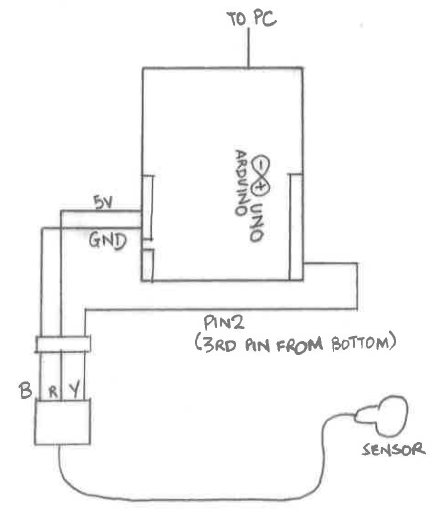
\includegraphics[width=0.5\textwidth]{../arduino_setup_yr19.png}
  \end{center}
  \end{figure}
  If you aren't sure, ask for help.
\item
  Connect the Arduino to one of the USB ports on the PC, and then
  double-click on the \texttt{hr2b.ino} program to open the Arduino IDE.
\item
  Once it is open, go to \emph{Tools \textgreater{} Port} and select the
  COM port that your Arduino Uno is connected to. Write it down
  (e.g.~COM4, or COM5 etc.) somewhere to remember it.
\item
  Clip the sensor onto the index finger on your non-master hand, and remain
  still. Ask one of your team to click on the magnifying glass icon on the top
  right of the Arduino program. You should see a new window pop up, with a number
  being printed continually. An LED on the Arduino should also blink each time
  this happens.
\end{enumerate}

\pagebreak

Take a look at the code in the Arduino window. What do you think it is
doing? What are the numbers being printed?

\vspace{1.5em}
\rule{16cm}{0.5pt}

\vspace{1.5em}
\rule{16cm}{0.5pt}

\vspace{1.5em}
\rule{16cm}{0.5pt}

Is the heart rate sensor working? How would you check?

\vspace{1.5em}
\rule{16cm}{0.5pt}

\vspace{1.5em}
\rule{16cm}{0.5pt}

\vspace{1.5em}
\rule{16cm}{0.5pt}

\hypertarget{jupyter-notebooks}{%
\subsection{Jupyter Notebooks}\label{jupyter-notebooks}}

\begin{enumerate}
\def\labelenumi{\arabic{enumi}.}
\tightlist
\item
  Open up the ``stats\_camp'' folder that is on the Desktop.
\item
  Press Shift and Right-click within this window (not on any particular file,
  just in the empty space). A menu should pop-up.  One of the options should be
  ``Open Powershell here''. Click on that.
\item
  In the terminal that opens, type in
\end{enumerate}
\begin{verbatim}
jupyter notebook
\end{verbatim}
\begin{enumerate}
\def\labelenumi{\arabic{enumi}.}
\setcounter{enumi}{3}
\tightlist
\item
  A browser tab should open, with the contents of the directory shown.
  Click on the \texttt{data\_capture.ipynb} file.
\end{enumerate}

What you see now is called a Jupyter notebook. It consists of Python
code, interspersed with comments and text. The code chunks are referred
to as cells. These are the sections that have the word 
\begin{verbatim}
In [6]: 
\end{verbatim}
on the left.

To run a cell, use the up and down arrow keys to navigate
to it, and then hit Ctrl-Enter.

\begin{enumerate}
\def\labelenumi{\arabic{enumi}.}
\setcounter{enumi}{4}
\tightlist
\item
  Run the first two cells now. You will not have to run these again
  through-out the session. These two cells import the relevant Python libraries
  for communicating with the Arduino, and instantiate a progress bar.
\item
  The next cell specifies the port that the Arduino is connected to, and the
  file to which you wish to save the data. The default filename that you see is
  ``testing\_output\_after\_exercise.txt''.

  Edit the lines in this cell (\textbf{Don't run the cell yet!}) to
  correspond to the COM port that you noted earlier. For instance, if it
  was COM5, then the line should be
\end{enumerate}

\begin{verbatim}
ser = serial.Serial('COM5')
\end{verbatim}
  Also, change the filename to which you wish to save the first batch of data.
  You will not have to change the COM port name for the rest of today, but you
  will have to change the filename for each person and each activity for which
  record the heart-rate. At this point, your cell might look like this:
\begin{verbatim}
In [8]: ser = serial.Serial('COM5')
        f=open('john_baseline.txt', 'w')
        total_time = 185
\end{verbatim}

\hypertarget{data-capture}{%
\section{Data Capture}\label{data-capture}}

Every data capture phase consists of the following steps:

\begin{enumerate}
\def\labelenumi{\arabic{enumi}.}
\tightlist
\item
  Edit the file name to correspond to your name and activity. For
  instance, you might change it from
  \texttt{testing\_output\_after\_exercise.txt} to
  \texttt{john\_baseline.txt}. Clip the sensor onto your non-master
  index finger, and then run this cell (underneath the \emph{Create
  Connections} heading) to initiate the capture.
\item
  Run the cell underneath the \emph{Start the capture} heading. This
  will begin the capture process. Each capture will take about 3
  minutes; you should see a progress bar each time. Be as still as 
  you can at this stage.
\item
  Run the cell underneath the \emph{Close all connections} heading. This
  will complete one data capture phase. You should see the new file in
  your directory. Check that it is not empty.
\end{enumerate}

If you encounter any errors, run the cell to close all connections, and then
start again from the first stpe in this section.

Today, each of you will capture data \emph{FOUR} times:

\begin{enumerate}
\def\labelenumi{\arabic{enumi}.}
\tightlist
\item
  Your baseline heart rate.
\item
  Your heart rate while watching the sports video at this link:
\begin{verbatim}
https://youtu.be/K148UvqF5zk
\end{verbatim}

\item
  Your heart rate while trying to solve a mathematics problem. It's ok if
  you cannot solve it; just try your best. If you solve it within 3
  minutes, just relax and wait for it to finish.
\item
  Our lab is on the fifth floor. Walk (do not run, please) down the
  stairs to the ground floor, then back to the lab and immediately
  capture your heart rate.
\end{enumerate}

\hypertarget{uploading}{%
\section{Uploading}\label{uploading}}

\begin{enumerate}
\def\labelenumi{\arabic{enumi}.}
\tightlist
\item
  In an \emph{new tab} in the browser, navigate to this address:
\end{enumerate}

\begin{verbatim}
http://sta93.stat.nus.edu.sg:8000/vik/data_upload
\end{verbatim}

\begin{enumerate}
\def\labelenumi{\arabic{enumi}.}
\setcounter{enumi}{1}
\tightlist
\item
  Make sure the files that were created are not empty before proceeding.
  Fill up the entries on the page accurately, select the appropriate activity and
  hit Upload, one file at a time.
\item
  The device id can be found on a sticker on the back of the Arduino.
  Please enter it in full, so it should be of the form ``Dxx''. If you are not
  sure about your person id, check with the instructor.
\item
  Please ensure that you input your weight (in kg) and height (in metres) 
  consistently. This
  is important in order to match the entries. If you made any incorrect
  entries, please inform one of the instructors.
\item
  Please upload the files in the activity order listed above, person by
  person. Take some time as you upload to think about the following:
\begin{itemize}
\item 
When you uploaded the baseline file, what do the two entries show? What
are the blue and red lines? What do you think is the difference between
the two plots? Make a note of your average resting heart rate here.

\vspace{1.5em}
\rule{16cm}{0.5pt}

\vspace{1.5em}
\rule{16cm}{0.5pt}

\vspace{1.5em}
\rule{16cm}{0.5pt}

\item 
When you uploaded the video and math files, what did you observe? Was
there a difference between this and your resting heart rate?

\vspace{1.5em}
\rule{16cm}{0.5pt}

\vspace{1.5em}
\rule{16cm}{0.5pt}

\vspace{1.5em}
\rule{16cm}{0.5pt}

\item 
When you upload the exercise file, try to estimate the time it took to
return to normal. Write down your recovery time (in seconds) here.

\vspace{1.5em}
\rule{16cm}{0.5pt}

\vspace{1.5em}
\rule{16cm}{0.5pt}

\vspace{1.5em}
\rule{16cm}{0.5pt}

\item 
Is it fair to use your personal guess as your recovery time? If not, how
can we automate this detection? What rule would you use? What is good
and what is bad about it?

\vspace{1.5em}
\rule{16cm}{0.5pt}

\vspace{1.5em}
\rule{16cm}{0.5pt}

\vspace{1.5em}
\rule{16cm}{0.5pt}

\end{itemize}

\end{enumerate}



\end{document}
